\documentclass[border=10pt]{standalone}
\usepackage{pgfplots}
\usepackage{tikz}
\usepgfplotslibrary{colormaps}
\pgfplotsset{trig format plots=rad}
\begin{document}
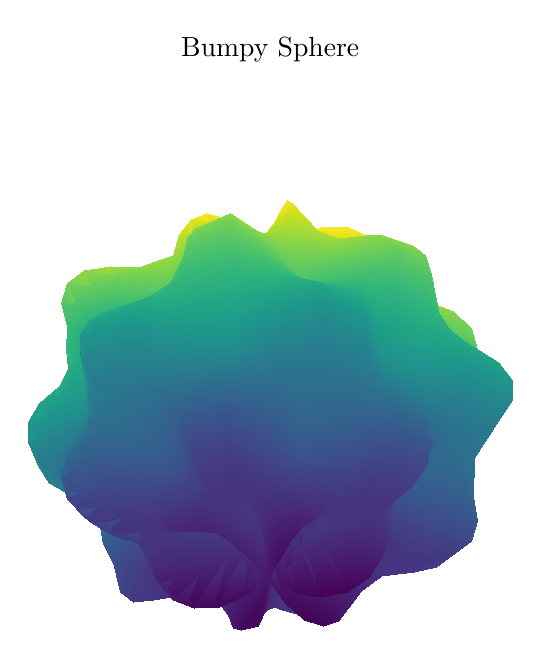
\begin{tikzpicture}
\begin{axis}[
    view={60}{30},
    width=10cm, height=10cm,
    axis lines=center,
    grid=major,
    colormap/viridis,
    title={Bumpy Sphere},
]
% To plot a 3D surface with many points, we need to sample.
% However, PGFplots is slow with large numbers of points.
% We will use a mesh of points.
\addplot3[surf, shader=interp, domain=0:6.28, domain y=0:3.14, samples=30, samples y=30] 
({(1 + 0.2*sin(6*x)*sin(5*y))*sin(y)*cos(x)}, 
 {(1 + 0.2*sin(6*x)*sin(5*y))*sin(y)*sin(x)}, 
 {(1 + 0.2*sin(6*x)*sin(5*y))*cos(y)});
\end{axis}
\end{tikzpicture}
\end{document}
